\chapter{Constrained optimization}
In the previous chapter, we draw the analogy between an optimization problem and the search for the lowest point in a mountainous landscape. We may continue with this analogy and make it a bit more realistic: \emph{Previously, the hiking person was able to access any point in the mountain range $\mathcal{S}$. However, in reality we might find a couple of constrains in that mountainous landscape. Someone might have put fences in the landscape and we are not able to cross these fences or we are restricted to a hiking path and cannot leave that path.}

These additional constraints make the optimization harder - the optimum that is achievable for us might be just "at a fence" and not the global optimum of the unrestricted function.
We denote the general form of a constrained optimization problem as 
\begin{equation}
    \begin{aligned}
        \min_{\mathbf{x}} \quad & f(\mathbf{x})\\
        \textrm{s.t.} \quad & g_i(\mathbf{x}) \le 0    &i \in [1, n]\\
                            & h_j(\mathbf{x}) = 0  &j \in [1, m]\\
                            & \mathbf{x} \in \mathcal{X} \subset \mathcal{R}^d\\
    \end{aligned}
    \label{eq:constrained_optimization}
\end{equation}
with $n$ inequality constraints $g_i : \mathcal{X} \rightarrow \mathcal{R}$ ("fences"), $m$ equality constraints $h_j: \mathcal{X} \rightarrow \mathcal{R}$ ("hiking paths") and a box constraint $\mathbf{x} \in \mathcal{X}$ ("allowed zone" in the mountain range). A constrained optimization problem is strictly convex, if the set $\mathcal{X}$ is strictly convex, the objective function is strictly convex and the constraints are strictly convex.

\begin{objectives}{}{objectives_constrained_optimization}
After studying this chapter and finishing the exercise, you should be able to 
\begin{itemize}[label=$\dots$]
    \item treat box constraints in gradient decent methods with projected gradients
    \item formulate Lagrangian functions of constrained optimization problems
    \item apply the Karush-Kuhn Tucker conditions to find the optimum of a convex constrained optimization problem
    \item explain the term \emph{Lagangian duality} and in which cases the dual formulation is beneficial
    \item apply the Langragian duality method to solve convex separable problems
\end{itemize}
\end{objectives}

\section{Box constraints} 
First, we neglect the equality constraints and inequality constraints in the problem \eqref{eq:constrained_optimization}, i.e. $m=0, n=0$, and focus on box constraints $\mathbf{x} \in \mathcal{X}$. \emph{Box constraint} means that the variables are limited to an upper and lower bound $\mathbf{x}^u$ and $\mathbf{x}^l$, respectively. For example, design variables in structural optimization could be diameters of beams, which cannot become negative or should not exceed a certain maximum producible size.

These constraints are probably the most friendly constraints in an optimization problem and in a one-dimensional optimization problem we can deal with them simply by clipping the variable as 
\begin{equation}
    x^* = \max(\min(\hat{x}, x^u), x^l)
\end{equation}
with the stationary point $\hat{x}$, the lower bound $x_l$ and the upper bound $x_u$. However, clipping the stationary point in each dimension of a multi-dimensional problem would not result in the optimal point, as illustrated by the green point in the next example \cite{Niculae2020}.

One method to deal with box constrains in multi-dimensional optimization problems is the projected gradient method. In this method we project each step of a gradient decent back to the domain as 
\begin{equation}
    \mathbf{x}^{k+1} = P(\mathbf{x}^k -\eta \nabla f(\mathbf{x}^k))
\end{equation}
with a projection function $P: \mathcal{R}^d \rightarrow \mathcal{X}$. In case of box constraints, this projection is simply clipping the values to $\mathcal{X}$ by 
\begin{equation}
    P(\mathbf{x}) = \max(\min(\mathbf{x}, \mathbf{x}^u), \mathbf{x}^l),
\end{equation}
where the $\max()$ and $\min()$ operators perform a point-wise comparison. 

\begin{example}{Box constraints}{boxexample}
    We want to find the solution of the following quadratic optimization problem
    \begin{equation}
        \begin{aligned}
            \min_{\mathbf{x}} \quad & f(\mathbf{x})= (\mathbf{x}-\tilde{\mathbf{x}}) \cdot \mathbf{Q} \cdot (\mathbf{x}-\tilde{\mathbf{x}})\\
            \textrm{s.t.} \quad     & \mathbf{x}^l \le \mathbf{x} \le \mathbf{x}^u\\
        \end{aligned}
        \label{eq:boxexample}
    \end{equation}
    with 
    \begin{equation}
        \mathbf{Q} = 
        \begin{pmatrix}
        2 & 1 \\
        1 & 1 
        \end{pmatrix}
        ,
        \tilde{\mathbf{x}} = 
        \begin{pmatrix}
        -1\\
        1 
        \end{pmatrix}
        ,
        \mathbf{x}^l = 
        \begin{pmatrix}
        0\\
        -2 
        \end{pmatrix}
        ,
        \mathbf{x}^u = 
        \begin{pmatrix}
        2\\
        2 
        \end{pmatrix}
        .
    \end{equation}

    \begin{center}
        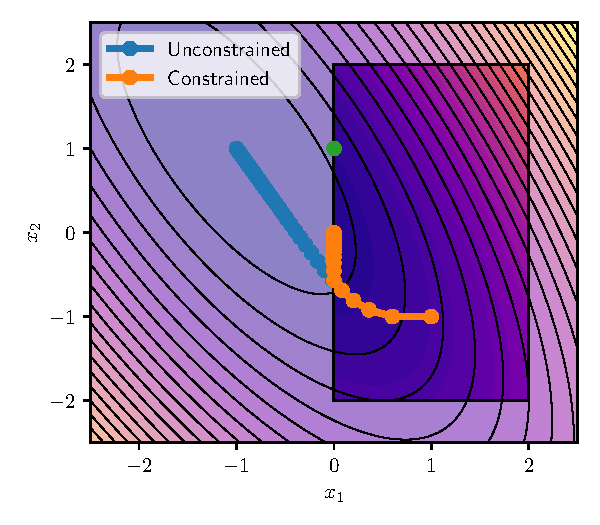
\includegraphics[width=0.5\textwidth]{figures/box_example.pdf}
    \end{center}

    This is visually equivalent to searching for that point $\mathbf{x}^*$ within the non-faded region in the displayed plot that has the smallest function value. In the unconstrained optimization problem, a simple steepest gradient decent follows the blue path and results in the blue point $(-1, 1)^\top$. In the constrained optimization problem, a simple steepest gradient decent follows the orange path and results in the orange point indicating the correct solution $(0, 0)^\top$ to problem \eqref{eq:boxexample}. Note that simply clipping the result $(-1, 1)^\top$ in each dimension would yield the position indicated by the green point, which is not the optimum.    
\end{example}


\section{Lagrange multipliers}
Now, we neglect only the inequality constraints in the problem \eqref{eq:constrained_optimization}, i.e. $n=0$. Then we can solve the problem using Lagrange multipliers. To do so, we formulate the Lagrangian function
\begin{equation}
    \mathcal{\mathcal{L}} (\mathbf{x}, \pmb{\lambda}) = f(\mathbf{x}) + \sum_{j=1}^m \lambda_j h_j(\mathbf{x}) 
\end{equation}
with so called Lagrangian multipliers $\pmb{\lambda} \in \mathcal{R}^m$. 
According to the Lagrange multiplier theorem, a stationary point of the Langrangian function 
\begin{align}
    \frac{\partial \mathcal{\mathcal{L}}}{\partial x_k} (\mathbf{x}^*, \pmb{\lambda}^*) &= \frac{\partial f }{\partial x_k} (\mathbf{x}^*) + \sum_{j=1}^m \lambda_j^* \frac{\partial h_j}{\partial x_k} (\mathbf{x}^*) = 0\\
    \frac{\partial \mathcal{\mathcal{L}}}{\partial \lambda_j} (\mathbf{x}^*, \pmb{\lambda}^*) &= h_j(\mathbf{x}^*) = 0,
\end{align}
fulfills the necessary condition to be an optimum of a constrained optimization problem, if the gradients of the equality constraints are linearly independent (\emph{Slater condition} or \emph{constraint qualification}). We may interpret these optimality conditions such that any directional derivative in a feasible direction becomes zero.

\begin{example}{Lagrange multipliers}{lagrangeexample}
    We want to find the solution of the following quadratic optimization problem for $\mathbf{x} \in \mathcal{R}^2$
    \begin{equation}
        \begin{aligned}
            \min_{\mathbf{x}} \quad & f(\mathbf{x})= (\mathbf{x}-\tilde{\mathbf{x}}) \cdot \mathbf{Q} \cdot (\mathbf{x}-\tilde{\mathbf{x}})\\
            \textrm{s.t.} \quad     & h(\mathbf{x}) = x_1 - x_2 - 2 = 0  \\
        \end{aligned}
    \end{equation}
    with 
    \begin{equation}
        \mathbf{Q} = 
        \begin{pmatrix}
        2 & 0 \\
        0 & 1 
        \end{pmatrix} 
        \quad 
        \text{and}
        \quad
        \tilde{\mathbf{x}} = 
        \begin{pmatrix}
        -1\\
        1 
        \end{pmatrix}.
    \end{equation}

    This is visually equivalent to searching for the point on the black line in the following image that has the smallest function value.
    \begin{center}
        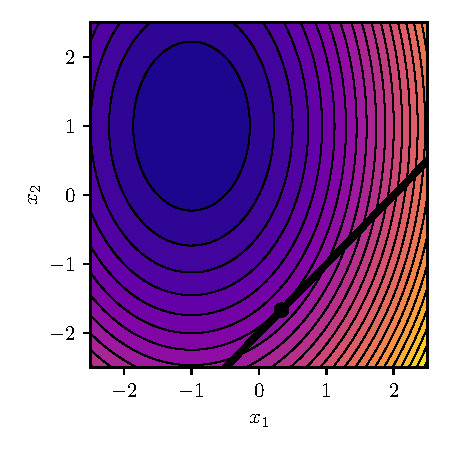
\includegraphics[width=0.5\textwidth]{figures/lagrange_example.pdf}
    \end{center}

    We can find the solution to this problem by finding a stationary point of the Lagrangian function
    \begin{equation}
        \mathcal{\mathcal{L}}(\mathbf{x}, \lambda) = 2 (x_1-\tilde{x}_1)^2 + (x_2-\tilde{x}_2)^2 + \lambda (x_1 - x_2 -2)
    \end{equation}
    with its partial derivatives 
    \begin{align}
        \frac{\partial \mathcal{\mathcal{L}}}{\partial x_1} &= 4 x_1^* + \lambda^*  + 4 = 0\\
        \frac{\partial \mathcal{\mathcal{L}}}{\partial x_2} &= 2 x_2^* - \lambda^*  -2 = 0\\
        \frac{\partial \mathcal{\mathcal{L}}}{\partial \lambda} &= x_1^* - x_2^* -2 = 0.
    \end{align}
    This is a linear system of three equations with three unknowns and we can easily find the solution $x_1^*=\frac{1}{3} , x_1^*=-\frac{5}{3}, \lambda^*=-\frac{16}{3}$
\end{example}


\section{Karush-Kuhn-Tucker conditions}
The Lagrange multipliers where initially only defined for equality constraints. However, the concept can be extended to inequality constraints with a Lagrangian function 
\begin{equation}
    \mathcal{\mathcal{L}} (\mathbf{x}, \pmb{\mu}, \pmb{\lambda}) = f(\mathbf{x}) + \sum_{i=1}^n \mu_i g_i(\mathbf{x}) + \sum_{j=1}^m \lambda_j h_j(\mathbf{x}) 
\end{equation}
utilizing the Lagrangian multipliers $\pmb{\mu} \in \mathcal{R}^n$ and $\pmb{\lambda} \in \mathcal{R}^m$ \cite{Karush1939, Kuhn1951}.

Assuming that the gradients of the constraints are linearly independent, we can then formulate the Karush-Kuhn-Tucker (KKT) conditions as necessary conditions for an optimum of the optimization problem \eqref{eq:unconstrained_optimzation}: 
\begin{align}
    \frac{\partial \mathcal{\mathcal{L}}}{\partial x_k} (\mathbf{x}^*, \pmb{\mu}^*, \pmb{\lambda}^*) &= 
    \frac{\partial f }{\partial x_k} (\mathbf{x}^*) + \sum_{j=1}^n \mu_i^* \frac{\partial g_i}{\partial x_k} (\mathbf{x}^*) + \sum_{j=1}^m \lambda_j^* \frac{\partial h_j}{\partial x_k} (\mathbf{x}^*) = 0 \\
    h_j(\mathbf{x}^*) &= 0 \quad j \in [1,m]\\
    g_i(\mathbf{x}^*) &\le 0 \quad i \in [1,n]\\
    \mu_i^* &\ge 0 \quad i \in [0,n] \\
    \mu_i^* g_i(\mathbf{x}^*) &=0 \quad i \in [1,n]
\end{align}
The first condition is the stationary condition, the next two conditions are the primal feasibility conditions, the next condition is the dual feasibility condition and the last condition is termed the complementary slackness condition. The slackness condition is either fulfilled by $\mu_i^*>0$ and $g_i(\mathbf{x}^*)=0$ for an active constraint or by  $\mu_i^*=0$ and $g_i(\mathbf{x}^*) \le 0$ for an inactive constraint \cite{Christensen2008, Harzheim2014}.

\begin{example}{Karush-Kuhn-Tucker conditions 1}{kktexample1}
    We want to find the solution of the following quadratic optimization problem for $\mathbf{x} \in \mathcal{R}^2$
    \begin{equation}
        \begin{aligned}
            \min_{\mathbf{x}} \quad & f(\mathbf{x})= (\mathbf{x}-\tilde{\mathbf{x}}) \cdot \mathbf{Q} \cdot (\mathbf{x}-\tilde{\mathbf{x}})\\
            \textrm{s.t.} \quad     & h(\mathbf{x}) = x_1 - x_2 - 2 = 0  \\
                          \quad     & g(\mathbf{x}) = x_1 + x_2 \le 0  \\
        \end{aligned}
    \end{equation}
    with 
    \begin{equation}
        \mathbf{Q} = 
        \begin{pmatrix}
        2 & 0 \\
        0 & 1 
        \end{pmatrix} 
        \quad 
        \text{and}
        \quad
        \tilde{\mathbf{x}} = 
        \begin{pmatrix}
        -1\\
        1 
        \end{pmatrix}.
    \end{equation}

    This is visually equivalent to searching for a point with the smallest function value on the black line that is within the non-faded area in the following image.
    \begin{center}
        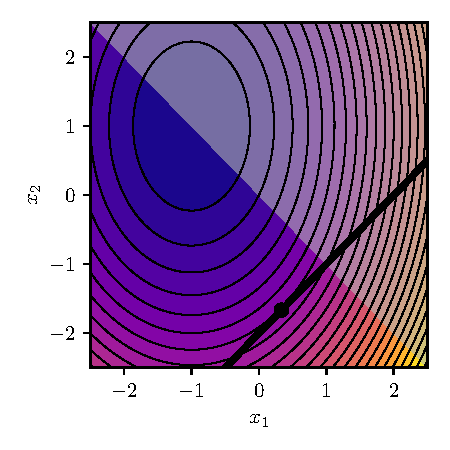
\includegraphics[width=0.5\textwidth]{figures/kkt_example_1.pdf}
    \end{center}

    The Lagrangian for this problem is 
    \begin{equation}
        \mathcal{\mathcal{L}}(\mathbf{x}, \mu, \lambda) = 2 (x_1-\tilde{x}_1)^2 + (x_2-\tilde{x}_2)^2 + \mu (x_1+x_2) + \lambda (x_1 - x_2 -2).
    \end{equation}

    The KKT conditions are 
    \begin{align}
        \frac{\partial \mathcal{\mathcal{L}}}{\partial x_1} &= 4 (x_1^* + 1) + \mu^* + \lambda^*  = 0\\
        \frac{\partial \mathcal{\mathcal{L}}}{\partial x_2} &= 2 (x_1^* - 1) + \mu^* - \lambda^*  = 0\\
        \frac{\partial \mathcal{\mathcal{L}}}{\partial \lambda} &= x_1^* - x_2^* - 2 = 0 \\
        \label{eq:kkt_example1_in}
        \frac{\partial \mathcal{\mathcal{L}}}{\partial \mu} &= x_1^*+x_2^* \le 0 \\
        \mu^* &\ge 0 \\
        0 &= \mu^*(x_1+x_2)
        \label{eq:kkt_example1_comp}
    \end{align}
    Obviously, the inequality constraint $g(\mathbf{x})$ is not active at $\mathbf{x}^*$, hence $\mu^*=0$ and Equations \eqref{eq:kkt_example1_in} to \eqref{eq:kkt_example1_comp} are fulfilled. The remaining problem is equivalent to the previous example.
\end{example}

\begin{example}{Karush-Kuhn-Tucker conditions 2}{kktexample2}
    We want to find the solution of the following quadratic optimization problem for $\mathbf{x} \in \mathcal{R}^2$
    \begin{equation}
        \begin{aligned}
            \min_{\mathbf{x}} \quad & f(\mathbf{x})= (\mathbf{x}-\tilde{\mathbf{x}}) \cdot \mathbf{Q} \cdot (\mathbf{x}-\tilde{\mathbf{x}})\\
            \textrm{s.t.} \quad     & h(\mathbf{x}) = x_1 - x_2 - 2 = 0  \\
                          \quad     & g(\mathbf{x}) = -x_1 - x_2 \le 0  \\
        \end{aligned}
    \end{equation}
    with 
    \begin{equation}
        \mathbf{Q} = 
        \begin{pmatrix}
        2 & 0 \\
        0 & 1 
        \end{pmatrix} 
        \quad 
        \text{and}
        \quad
        \tilde{\mathbf{x}} = 
        \begin{pmatrix}
        -1\\
        1 
        \end{pmatrix}.
    \end{equation}

    This is visually equivalent to searching for a point with the smallest function value on the black line that is within the non-faded area in the following image.
    \begin{center}
        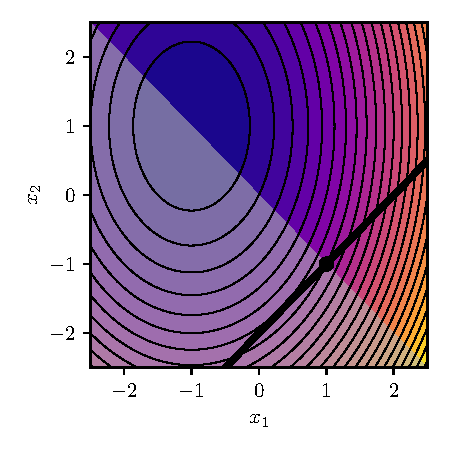
\includegraphics[width=0.5\textwidth]{figures/kkt_example_2.pdf}
    \end{center}

    The Lagrangian for this problem is 
    \begin{equation}
        \mathcal{\mathcal{L}}(\mathbf{x}, \mu, \lambda) = 2 (x_1-\tilde{x}_1)^2 + (x_2-\tilde{x}_2)^2 - \mu (x_1+x_2) + \lambda (x_1 - x_2 -2).
    \end{equation}

    The KKT conditions are 
    \begin{align}
        \frac{\partial \mathcal{\mathcal{L}}}{\partial x_1} &= 4 (x_1^* + 1) - \mu^* + \lambda^*  = 0\\
        \frac{\partial \mathcal{\mathcal{L}}}{\partial x_2} &= 2 (x_2^* - 1) - \mu^* - \lambda^*  = 0\\
        \frac{\partial \mathcal{\mathcal{L}}}{\partial \lambda} &= x_1^* - x_2^* - 2 = 0 \\
        \label{eq:kkt_example2_in}
        \frac{\partial \mathcal{\mathcal{L}}}{\partial \mu} &= -x_1^*-x_2^* \le 0 \\
        \mu^* &\ge 0 \\
        0 &= \mu^*(-x_1-x_2)
        \label{eq:kkt_example2_comp}
    \end{align}
    In this case, the inequality constraint $g(\mathbf{x})$ is active at $\mathbf{x}^*$, hence $\mu^* > 0$ and $g(\mathbf{x})=0$. This is used to eliminate the inequalities and leaves us with a linear system of equations 
    \begin{equation}
        \begin{pmatrix}
        4  & 0  & -1 & 1  \\
        0  & 2  & -1 & -1 \\ 
        1  & -1 & 0  & 0  \\
        -1 & -1 & 0  & 0
        \end{pmatrix} 
        \begin{pmatrix}
        x_1^* \\ x_2^* \\ \lambda^* \\ \mu^*  
        \end{pmatrix} 
        = 
        \begin{pmatrix}
        -4 \\ 2 \\ 2\\ 0
        \end{pmatrix} 
        .
    \end{equation}
    The solution of that system is $x_1^*=1$, $x_2^*=-1$, $\mu^*=2$, $\lambda^*=-6$.
\end{example}

\section{Lagrangian duality}
The examples in the previous sections could be solved with linear systems of equations, because the objective function was quadratic and the constraints were linear. In general, we need to employ an iterative solution method to obtain the results for non-linear optimization problems. 

However, we cannot use the gradient decent schemes directly, because the fact that the Lagrangian function becomes stationary at the optimum does not mean that this is a minimum. In fact, the stationary point of the Lagrangian is a saddle point (see Figure \ref{fig:saddle_point}), i.e. it is a minimum w.r.t. to the design variables and a maximum w.r.t. the Lagrange multipliers.

\begin{figure}[!htpb]
    \centering
    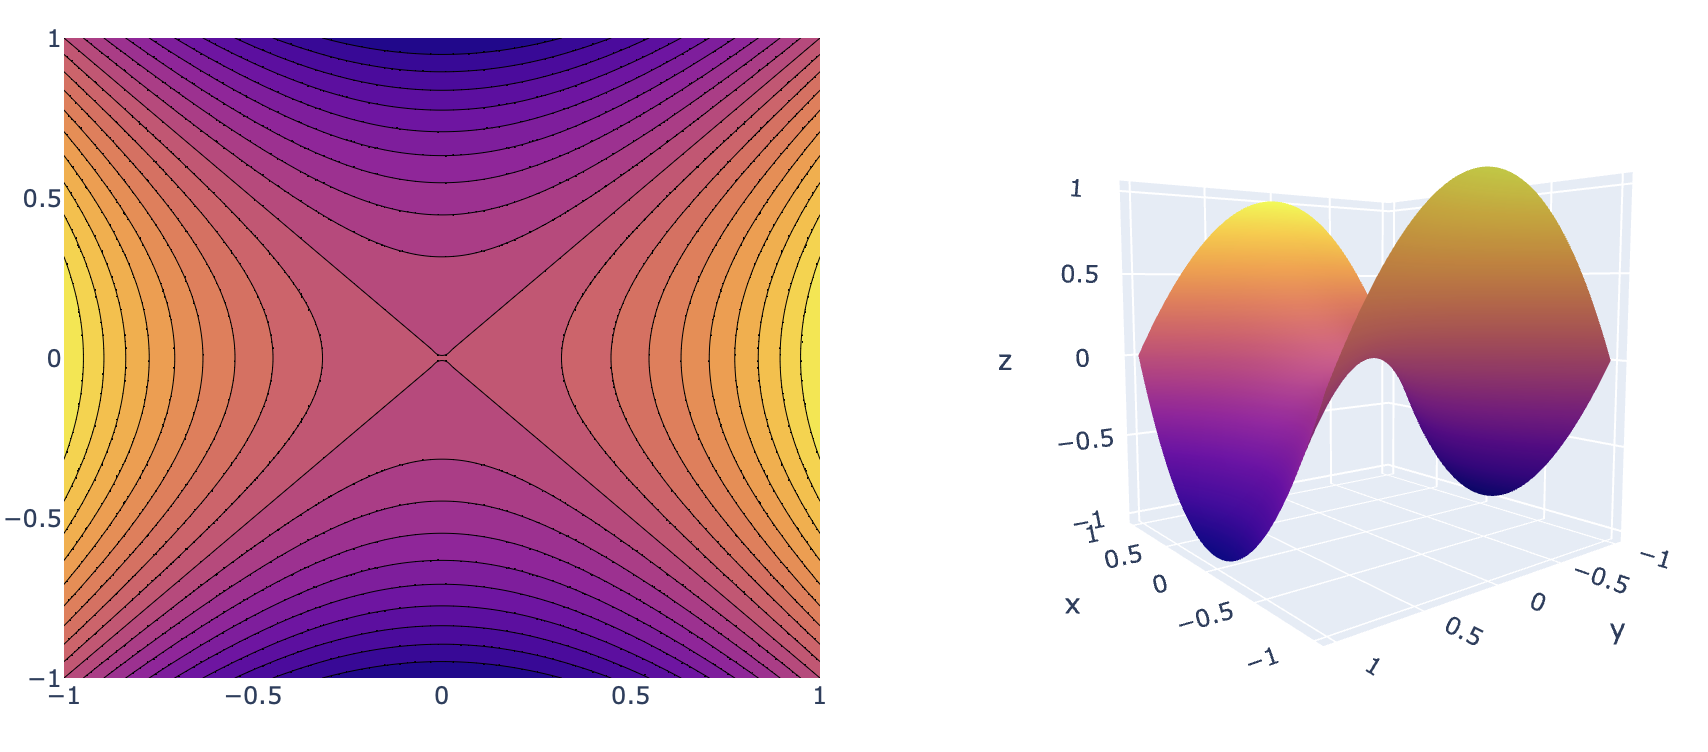
\includegraphics[width=\textwidth]{figures/saddle_point.png}
    \caption{Example of the contours and a 3D surface plot of a saddle point for $\mathbf{x} \in \mathcal{R}^2$.}
    \label{fig:saddle_point}
\end{figure}

One option to find the saddle point is called the \emph{primal method}, where the Lagrangian is first maximized w.r.t. $\pmb{\mu}$ and $\pmb{\lambda}$ with fixed $\mathbf{x}$ and subsequently minimized w.r.t. $\mathbf{x}$. Visually this is a decent along the ridge until we reach the saddle point. 
This formulation 
\begin{equation}
    \min_{\mathbf{x} \in \mathcal{X}} \underbrace{\max_{\pmb{\mu},\pmb{\lambda}} \mathcal{\mathcal{L}}(\pmb{\mu}, \pmb{\lambda}, \mathbf{x})}_{\bar{\mathcal{\mathcal{L}}}(\mathbf{x})}
\end{equation}
does not provide any helpful improvement, because the inner term $\bar{\mathcal{\mathcal{L}}}(\mathbf{x})$ just states the constraints 
\begin{align}
    \frac{\partial \mathcal{\mathcal{L}}}{\partial \mu_i} &= g_i(\mathbf{x}) = 0 \quad i \in \mathcal{I}\\
    \frac{\partial \mathcal{\mathcal{L}}}{\partial \lambda_j} &= h_j(\mathbf{x}) = 0 \quad j \in [1,m]
\end{align}
with $\mathcal{I}$ denoting the set of active inequality constraints. This leaves us with the same problem as \eqref{eq:constrained_optimization} and not much has been gained. 

However, it can be proven that for convex problems with linearly independent inequality constraints, we can invert the process and minimize the Lagrangian function w.r.t. $\mathbf{x}$ first and then maximize it w.r.t. $\pmb{\mu}$ and $\pmb{\lambda}$. Visually this is a maximization along the valley floor until we reach the saddle point \cite{Harzheim2014}. The formulation 
\begin{equation}
     \max_{\pmb{\mu},\pmb{\lambda}} \underbrace{\min_{\mathbf{x}\in \mathcal{X}} \mathcal{\mathcal{L}}(\pmb{\mu}, \pmb{\lambda}, \mathbf{x})}_{\underline{\mathcal{\mathcal{L}}} (\pmb{\mu}, \pmb{\lambda})}
\end{equation}
is helpful, because we are left with very simple box constraints in these optimization problems ($\mathbf{x} \in \mathcal{X}$ in the inner minimization and $\pmb{\mu} \ge 0$ in the maximization). 

\begin{example}{Dual problem}{dualityexample}
    We want to find the solution of the following quadratic optimization problem for $\mathbf{x} \in \mathcal{R}^2$
    \begin{equation}
        \begin{aligned}
            \min_{\mathbf{x}} \quad & f(\mathbf{x})= (\mathbf{x}-\tilde{\mathbf{x}}) \cdot \mathbf{Q} \cdot (\mathbf{x}-\tilde{\mathbf{x}})\\
            \textrm{s.t.} \quad     & h(\mathbf{x}) = (x_1+1)^2 + x_2 = 0  \\
        \end{aligned}
    \end{equation}
    with 
    \begin{equation}
        \mathbf{Q} = 
        \begin{pmatrix}
        2 & 0 \\
        0 & 1 
        \end{pmatrix} 
        \quad 
        \text{and}
        \quad
        \tilde{\mathbf{x}} = 
        \begin{pmatrix}
        -1\\
        1 
        \end{pmatrix}.
    \end{equation}

    This is visually equivalent to searching for a point on the black line in the following image that has the smallest function value.
    \begin{center}
        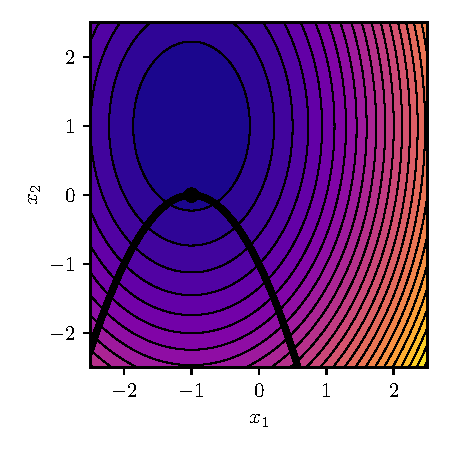
\includegraphics[width=0.5\textwidth]{figures/dual_example.pdf}
    \end{center}

    We can formulate the Lagrangian function as
    \begin{equation}
        \mathcal{\mathcal{L}}(\mathbf{x}, \lambda) = 2 (x_1-\tilde{x}_1)^2 + (x_2-\tilde{x}_2)^2 + \lambda \left[(x_1+1)^2 + x_2 \right].
    \end{equation}
    Now, we solve the dual problem by first minimizing the Lagrange function w.r.t. $\mathbf{x}$. For the stationary point, 
    \begin{align}
        \frac{\partial \mathcal{L}}{\partial x_1} &= 4 x^*_1 +4 + 2 \lambda x^*_1 + 2 \lambda = 0\\
        \frac{\partial \mathcal{L}}{\partial x_2} &= 2 x^*_2 - 2 + \lambda = 0
    \end{align} 
    applies. Hence, we can substitute 
    \begin{align}
        x^*_1(\lambda) = -1 \\
        x^*_2(\lambda) = 1 - \frac{1}{2} \lambda 
    \end{align}
    in $\mathcal{L}$ to obtain the dual objective function $\underline{\mathcal{L}} (\lambda)$. Now, we are left with a problem 
    \begin{equation}
        \max_{\lambda} \underline{\mathcal{L}} (\lambda) = 
        \max_{\lambda} \left( - \frac{\lambda^2}{4} + \lambda + \frac{1}{4} \right).
    \end{equation}
    The maximum is located at a stationary point, so with 
    \begin{equation}
        \frac{\partial \underline{\mathcal{L}} }{\partial \lambda} = 1 - \frac{\lambda^*}{2}  = 0
    \end{equation}
    we get $\lambda^*=2$, $x_1^*=-1$ and $x_2^*=0$.
\end{example}

The example shows that we need to be able to express the design variables $\mathbf{x}$ in terms of the Lagrangian variables in order to apply the dual method. This is typically not applicable to general optimization problems. However, the dual method is very attractive for \emph{separable} convex optimization problems, i.e. if the objective function can be expressed as 
\begin{equation}
    f(\mathbf{x}) = f_0 + \sum_{k=1}^d f_k(x_k)
\end{equation}
and the constraints can be expressed as 
\begin{align}
    g_i(\mathbf{x}) & = g_{i0} + \sum_{k=1}^d g_{ik}(x_k) \quad i \in [1,n]\\
    h_j(\mathbf{x}) & = h_{j0} + \sum_{k=1}^d h_{jk}(x_k) \quad j \in [1,m].
\end{align}
Then, the Lagrangian becomes 
\begin{equation}
    \mathcal{L} (\mathbf{x}, \pmb{\mu}, \pmb{\lambda}) = f_0 + \sum_{k=1}^d f_i(x_k) + \sum_{i=1}^n \mu_i \left(g_{i0} + \sum_{k=1}^d g_{ik}(x_k) \right) + \sum_{j=1}^m \lambda_j  \left(h_{j0} + \sum_{k=1}^d h_{jk}(x_k) \right)
\end{equation}
and is also separable
\begin{equation}
    \mathcal{L} (\mathbf{x}, \pmb{\mu}, \pmb{\lambda}) = \mathcal{L}_0 + \sum_{k=1}^d \mathcal{L}_k(x_k)
\end{equation}
with 
\begin{align}
    \mathcal{L}_0 &= f_0 + \sum_{i=1}^n \mu_i g_{i0} + \sum_{j=1}^m \lambda_j  h_{j0} \\
    \mathcal{L}_k (x_k) & = f_k(x_k) + \sum_{i=1}^n \mu_i g_{ik}(x_k) + \sum_{j=1}^m \lambda_j  h_{jk}(x_k). 
\end{align}
For such a separable convex problem, the search for the the "valley floor" 
\begin{equation}
    \min_{\mathbf{x}\in \mathcal{X}} \mathcal{L}(\pmb{\mu}, \pmb{\lambda}, \mathbf{x})
\end{equation} 
turns into $d$ simple strictly convex optimization problems 
\begin{equation}
    \min_{x_k \in [x_k^l, x_k^u]} \mathcal{L}_k(x_k) \quad k \in[1,d]
\end{equation}
which have a unique solution and are simple to solve because each of them is just a box-constrained single variable optimization problem. 
After finding the expression for $\underline{\mathcal{L}} (\pmb{\mu}, \pmb{\lambda})$ easily, we only need to solve this remaining problem $\max_{\pmb{\mu}, \pmb{\lambda}} \underline{\mathcal{L}} (\pmb{\mu}, \pmb{\lambda})$ w.r.t. $\pmb{\mu}$ and $\pmb{\lambda}$. The dual problem is therefore especially well suited for separable convex problems with $d \gg n+m$, i.e. for problems with many design variables and just a few constraints. This is typically the case for topology optimization.

\begin{example}{Separable problem}{separableexample}
    Let's consider the previous example with the additional constraint $\mathbf{x} \in \mathcal{X} = [0, 2]\times[-2, 2]$.
    This is visually equivalent to searching within the gray box for a point on the black line that has the smallest function value in the following image.
    \begin{center}
        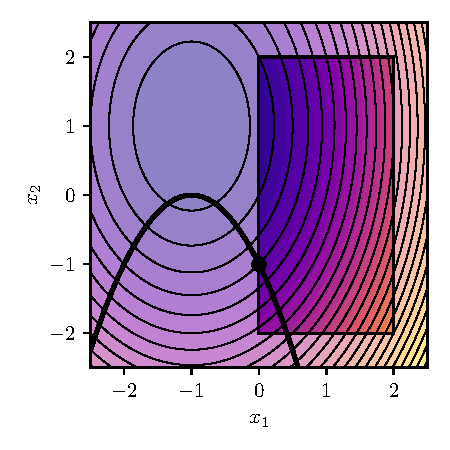
\includegraphics[width=0.5\textwidth]{figures/separable_example.pdf}
    \end{center}

    It would be tedious to solve the problem with additional inequality constraints like $g_1= x_1, g_2=x_1-2, g_3=x_2-2, g_4=2-x_2$. 

    However, we can formulate a separable Lagrangian function as
    \begin{equation}
        \mathcal{L}(\mathbf{x}, \lambda) = \underbrace{2 (x_1-\tilde{x}_1)^2 + \lambda (x_1+1)^2}_{\mathcal{L}_1(x_1)} + \underbrace{(x_2-\tilde{x}_2)^2  + \lambda x_2}_{\mathcal{L}_2(x_2)}.
    \end{equation}
    and can take care of box constraints trivially in each optimization by clipping. Using the stationary points 
    \begin{align}
        \frac{\partial \mathcal{L}_1}{\partial x_1} &= 4\hat{x}_1+4+2\lambda \hat{x}_1 + 2 \lambda = 0 \\
        \frac{\partial \mathcal{L}_2}{\partial x_2} &= 2\hat{x}_2-2+\lambda = 0
    \end{align}
    we can solve 
    \begin{align}
        x_1^*(\lambda) = \max(\min(\hat{x}_1(\lambda), x_1^u), x_1^l) &= 0 \\
        x_2^*(\lambda) = \max(\min(\hat{x}_2(\lambda), x_2^u), x_2^l) &= 
        \begin{cases}
            2 & \quad \lambda < -2 \\
            -2 & \quad \lambda > 6 \\
            1 - \frac{\lambda}{2} & \quad \text{else}
        \end{cases}
    \end{align}
    and the dual objective function becomes 
    \begin{equation}
        \underline{\mathcal{L}}(\lambda) = 
        \begin{cases}
            3 + 3 \lambda  & \quad \lambda < -2 \\
            11 - \lambda  & \quad \lambda > 6 \\
            2 + 2 \lambda - \frac{\lambda^2}{4}   & \quad \text{else.}
        \end{cases}
    \end{equation}
    This dual objective function is plotted here:
    \begin{center}
        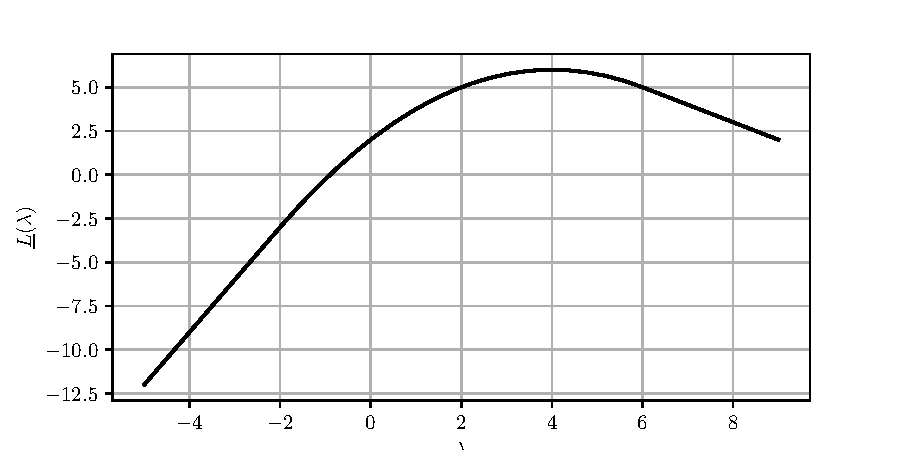
\includegraphics[width=\textwidth]{figures/dual_function.pdf}
    \end{center}
    We can employ any gradient decent method or analytical method to find the optimum of the dual function. In this case, it is $\lambda^*=4$ and therefore the optimum is at $x_1^*=0$ and $x_2^*=-1$.    
\end{example}

\bibliographystyle{unsrtnat}
\bibliography{literature} 